\section{Umsetzung}
Im Folgenden wird die Umsetzung insbesondere im
Bezug auf die Wahl der Technologie des Layouts
sowie Darstellung der App betrachtet.

\subsection{Technologie}
Um Apps zu entwickeln gibt es viele Möglichkeiten.
Diese lassen sich grob in folgende Arten einteilen

\begin{table}[htbp]
    \begin{tabular}{|l|l|}
    \hline
    Art      & Charakteristik                                                                                                                                                       \\ \hline
    Hybrid   & Web-Apps werden im nativen Kontext in einer WebView eingebunden                                                                                                      \\ \hline
    Native   & \begin{tabular}[c]{@{}l@{}}Adressieren konkrete Zielplattformen und deren Programmiersprachen.\\ Android (Java, Kotlin, Dart), iOS (Objective-C, Swift)\end{tabular} \\ \hline
    Web Apps & Über einen Server bereitgestellte plattformunabhängige Anwendungen                                                                                                   \\ \hline
    \end{tabular}
    \caption{Übersicht Arten von Apps}
\end{table}

Ich bin großer Fan von \ac{WORA} und entwickle üblicherweise vor allem Web-Apps.
Um etwas neues zu lernen und daran zu wachsen, entschied ich mich,
dieses Mal dazu eine Cross-Plattform-Technologie zu nutzen.
Die Entscheidung fiel dabei auf das von Google entwickelte Open Source \ac{UI}-Kit \textit{Flutter}.

\begin{figure}[H]
    \minipage[t]{0.4\textwidth}
        
\includegraphics[width=\linewidth]{flutter_logo}
        \caption{ Flutter-Logo }
    \endminipage\hfill
    \minipage[t]{0.4\textwidth}
        
\includegraphics[width=\linewidth]{dart_logo}
        \caption{ Dart-Logo }
    \endminipage\hfill
\end{figure}

\subsection{Besonderheiten von Flutter}
\subsubsection{Performance}
Eine der Besonderheiten von \textit{Flutter} ist es, dass dieses UI-Kit weder eine WebView
noch die vom Betriebssystem mitgelieferten Widgets benutzt. Widgets sind in der
Welt von \textit{Flutter} alles von Bedienelemente bis hin zu Layout-Helfern.
Statt diese mitgelieferten Widgets zu nutzen, setzt \textit{Flutter} auf eine
eigene Rendering-Engine welche häufig mit einer 2D-Spiele-Engine verglichen wird.
Eines der Entwicklungsziele von \textit{Flutter} war es nämlich,
besonders performante Apps entwickeln zu können welche mit einer hohen
Hertz-Zahl (60-120 \textit{Hz}) laufen. Mit diesem Ansatz ist es möglich,
die gesamte UI über den Grafikchip des Systems zu berechnen und die CPU zu entlassen.
Dadurch wird es außerdem möglich, Änderungen die man im Code vornimmt,
nahezu ohne Verzögerung in der App zu sehen, ohne das ein Neuladen oder ähnliches
notwendig ist.

\subsubsection{Dart}
\textit{Flutter}-Apps werden in der Programmiersprache \textit{Dart}
entwickelt. \textit{Dart} ist eine objektorientierte,
klassenbasierte Sprache mit Garbage-Collector und wird vor allem durch
\textit{Google} entwickelt. Sie wurde vor allem durch
\textit{C\#, Erlang, JavaScript, Smalltalk} sowie \textit{Strongtalk}
beeinflusst. Im \textit{Dart}-\ac{SDK} enthaltenen sind:
die \textit{Dart}-\ac{VM}, dem Compiler \textit{dart2js}
welcher es erlaubt \textit{Dart} in \textit{JavaScript}
zu kompilieren sowie der Paketmanager \textit{Pub}.
\textit{Dart}-Code kann mittels \ac{AOT} kompiliert werden.
Dies hat zum Vorteil das Programmcode vor der Ausführung in native
Maschinensprache übersetzt wird und somit wesentlich schneller ausgeführt
werden kann. Apps geschrieben mit \textit{Flutter} werden automatisch
per \textit{AOT} kompiliert.

\subsubsection{Deklaratives UI}
Im Gegensatz zu imperativen Frameworks wie dem \textit{Android SDK}
oder dem \textit{iOS UiKit} handelt es sich bei \textit{Flutter} um
ein so genanntes deklaratives Framework. Dies bedeutet,
dass das UI von Flutter immer akutellen \textit{"State"} reflektiert.
Wird beispielsweise eine Option in den Einstellungen einer App geändert,
so ändert sich der \textit{"State"} der App welches das Neuzeichnen
der App auslöst (eine Checkbox wird gefüllt, ein Switch aktiviert).
Imperativ würde bedeuten, dass es Methoden wie \textit{widget.setText}
gibt um Werte direkt zu ändern. Hier wird der \textit{"State"} geändert
und das UI wird komplett neu gezeichnet.

\paragraph{Technisches Beispiel}\mbox{}
\hfill
\break

\begin{figure}[H]
    \centering
    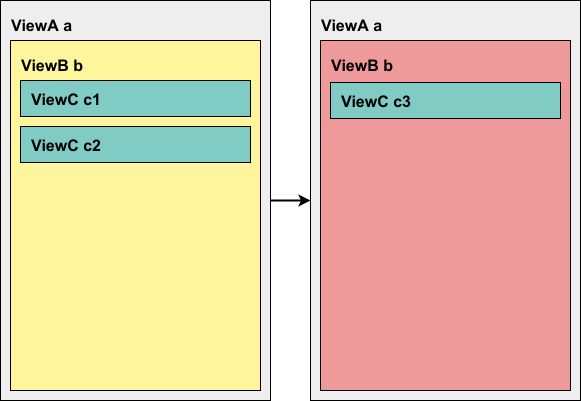
\includegraphics[width=0.8\columnwidth]{declarative_ui_example}
    \caption{Vergleich deklaratives \& imperatives UI}
\end{figure}

Im imperativen Stil würde man eine Instanz \textit{b} des so
genannten \textit{Owners} der View \textit{ViewB} nutzen
und mit Hilfe eine Selektors wie beispielsweise \textit{findViewById}
Änderungen auf dieser anwenden (und somit diese implizit invalidieren).
Das kann ungefähr so aussehen:

\begin{figure}[H]
    \centering
    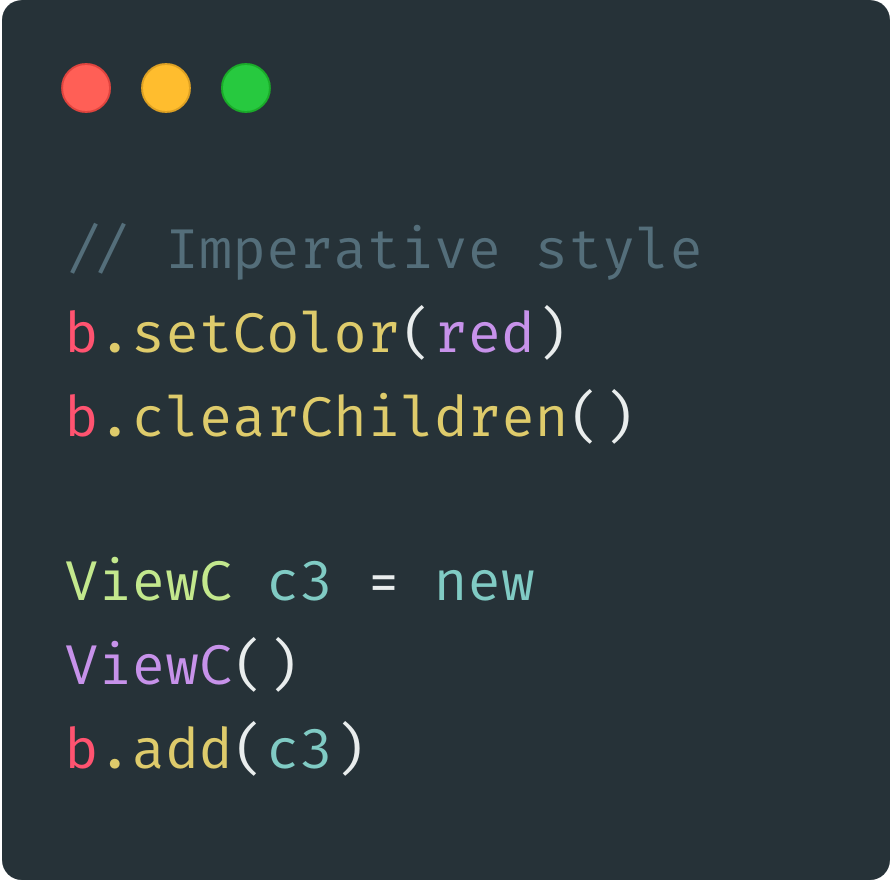
\includegraphics[width=0.4\columnwidth]{imperative_style}
    \caption{Beispiel: imperativer Stil}
\end{figure}

Außerdem müsste dieses Setup im Konstruktor von \textit{ViewB} dupliziert
werden, da die UI (der \ac{SPOT}) möglicherweise die Instanz \textit{b} überlebt.
Im deklarativen Frameworks sind View-Konfigurationen
(wie \textit{Flutter's} Widgets) unveränderlich (immutable) und an sich
nur simple Blaupausen. Um ein UI zu ändern, löst ein Widget einen Rebuild
auf sich selbst aus (in \textit{StatefulWidgets} häufig per \textit{setState()}
und erzeugt damit einen neuen Widget-Subtree.

\begin{figure}[H]
    \centering
    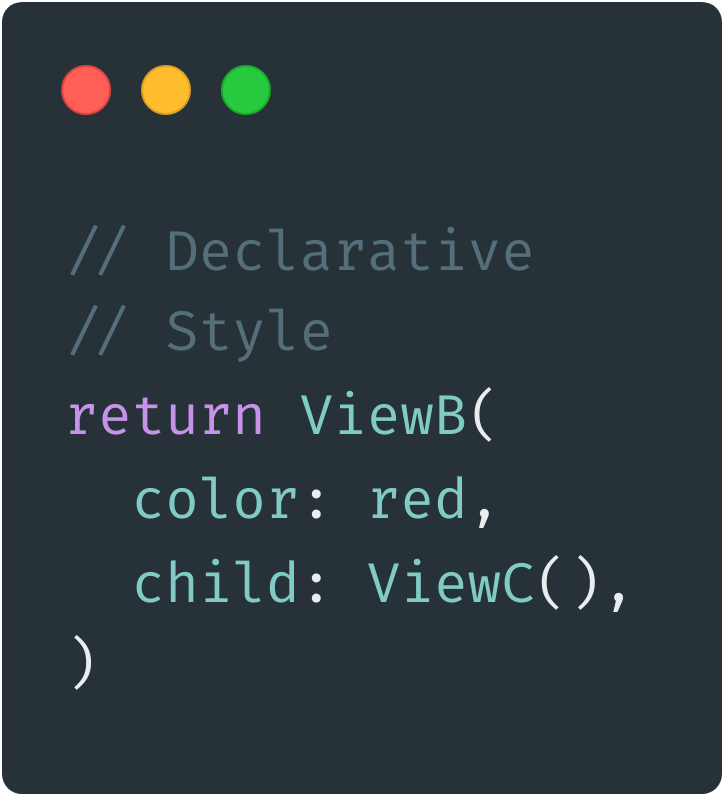
\includegraphics[width=0.4\columnwidth]{declarative_style}
    \caption{Beispiel: deklarativer Stil}
\end{figure}



\subsection{Herausforderungen}

Die folgenden Abschnitte zeigen Auszüge, die sich bei der Entwicklung
als besonders anspruchsvoll herausgestellt haben.

\subsubsection{Layout \& Design}

Die App besteht grundsätzlich aus drei Bereichen:
einer Liste, einem Informations-Panel und einem Formular.
Diese Bereiche sollen nahtlos ineinander übergehen um ein
möglichst professionellen Gesamteindruck zu vermitteln.
Das finale Layout entspricht in der Hauptansicht der untenstehenden Grafik.

\begin{figure}[H]
    \minipage[t]{0.4\textwidth}\vspace{0pt}
        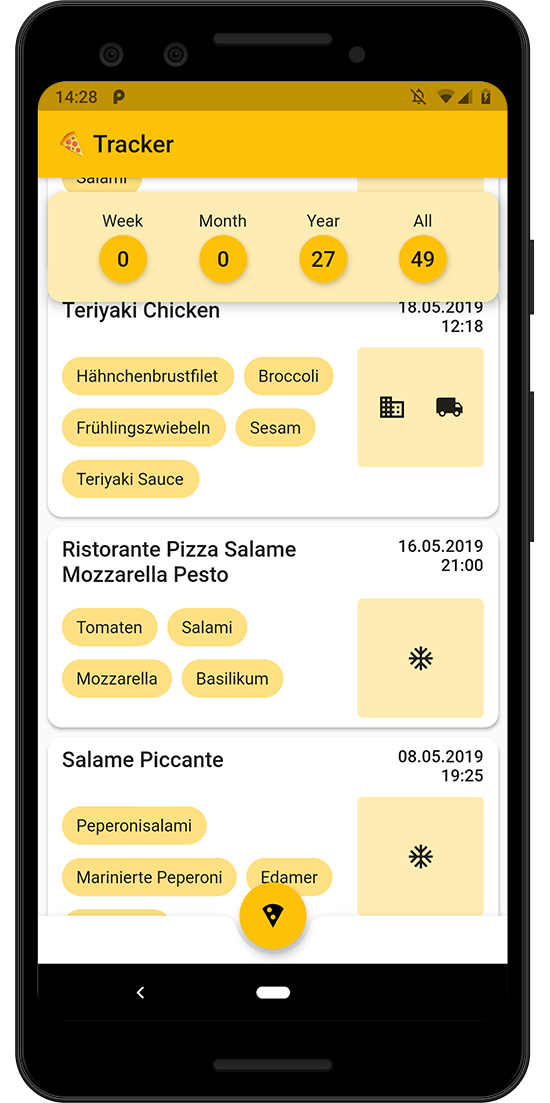
\includegraphics[width=\linewidth]{pixel-3_mockup-1}
        \caption{
            App: Hauptansicht
        }
    \endminipage\hfill
    \minipage[t]{0.6\textwidth}\vspace{0pt}
        Die Anordnung von Elementen erfolgt bei Flutter wie im Web:
        Die Reihenfolge im Quellcode gibt zugleich deren Reihenfolge auf
        der Y-Achse an. Elemente können sich dabei (auf der Z-Achse)
        nicht überlagern. Um Elemente übereinander darzustellen gibt es
        im Web die Property \textit{z-index}, in Flutter nutzt man das Widget
        \textit{Stack}. Im Stack-Widget ist das erste Element das auf der
        Z-Achse niedrigste Element. Grundsätzlich lassen sich viele
        Layout-Konzepte aus dem Web in Flutter übertragen. So gibt es
        Widgets wie \textit{Row, Column, Grid, Flex und Expanded} welche
        in ihrer Funktionalität gleich ihren Web-Pendants entsprechen.
        Interessant ist, dass \textit{Row} allerdings nicht umbricht,
        sobald zu viele Elemente in einer Zeile vorhanden sind und man
        für diesen Fall das Widget \textit{Wrap} benutzen muss.
        Grundsätzlich bietet Flutter eine große Auswahl an Widgets, die über
        reine Layout-Funktionalitäten hinaus gehen und optische Standardwerte
        mit sich bringen. So gibt es das \textit{Card}-Widget welches über
        dessen Properties \textit{elevation} und \textit{shape} einfache
        Mittel bereitstellt, um die Material-Design-typischen Schatten
        und abgerundeten Ecken zu erzielen.

    \endminipage\hfill
\end{figure}
Um nicht nur am oberen, sondern auch am unteren Ende der App
(am sogenannten \ac{FAB}) ein \textit{Überfließen} zu erzielen,
muss die Fläche der Liste auf die komplette Höhe des
Bildschirms erweitert werden.

\begin{figure}[H]
    \minipage[t]{0.4\textwidth}\vspace{0pt}
        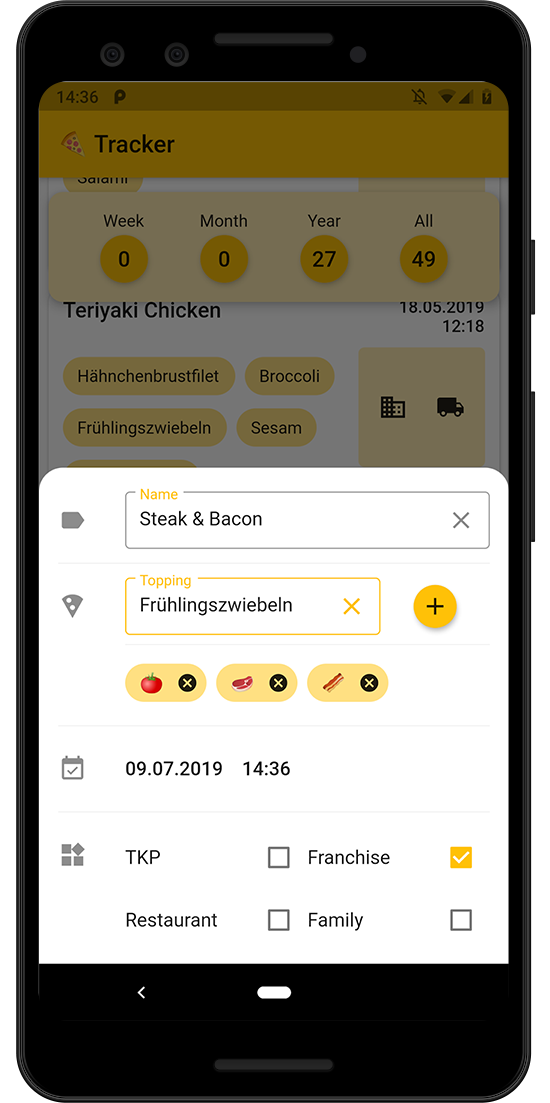
\includegraphics[width=\linewidth]{pixel-3_mockup-2--form}
        \caption{
            App: Formular
        }
    \endminipage\hfill
    \minipage[t]{0.6\textwidth}\vspace{0pt}
        Das Formular an sich besteht mehreren, grundsätzlich
        unabhängigen, Widgets:

        \begin{itemize}
            \itemsep-0.4em
            \item Name
            \item Toppings
            \item Datum \& Uhrzeit
            \item Art der Pizza:
            \begin{itemize}
                \itemsep-0.4em
                \item \ac{TKP}
                \item Franchise
                \item Restaurant
                \item Family
                \item Delivery
                \item Selfmade
            \end{itemize}
            \item Ort an dem die Pizza gegessen wurde
        \end{itemize}

        Hierbei stellten sich vor allem die Widgets für die
        Eingabe der Toppings und der Art der Pizza als besonders
        anspruchsvoll heraus. Bei den Toppings kam zum einen
        zwei Mal das \textit{Row}-, ein Mal das \textit{Wrap}
        sowie für die Toppings selbst das \textit{Chip}-
        (mit \textit{onDeleted}-Methode), bei der
        Art der Pizza vor allem das \textit{Grid}- sowie
        das \textit{Checkbox}- (in Kombination) mit dem \textit{Text}-Widget
        zum Einsatz.
    \endminipage\hfill
\end{figure}
Um im Formular abgerundete Ecken darstellen zu können, benötigt man
das extern erhältliche Widget \textit{showRoundedModalBottomSheet}.
Allerdings kann auch dieses nicht über eine Höhe von 50\% des Bildschirms
hinaus gehen und zwingt einen somit zum scrollen.

\begin{figure}[H]
    \centering
    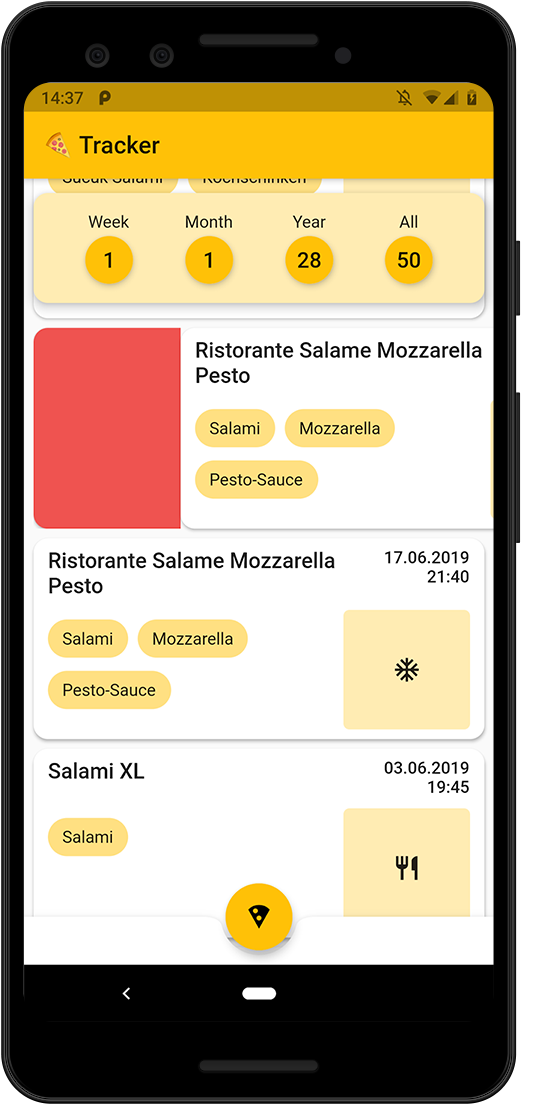
\includegraphics[width=0.4\columnwidth]{pixel-3_mockup-3--dismissible}
    \caption{App: Dismissible}
\end{figure}

Um Pizzen schnell wieder löschen (und später potentiell bearbeiten)
zu können, bietet sich das \textit{Dismissible}-Widget an.
Dieses kann man beliebig um andere Widgets packen und diesem
durch wischen in bestimmte Richtungen verschiedene Aktionen zuweisen.

\subsubsection{State-Management}


\subsubsection{Date-Library}

Um Filter für die verschiedenen Zeiträume setzen zu können,
ist es notwendig, ausgehend vom jetzigen Zeitpunkt,
den jeweiligen Start- und Endpunkt eines Zeitraums zu ermitteln.
Wichtig bei der Berechnung von Zeiträumen ist unter anderem auch
die korrekte Einbeziehung der Umstellung von Sommer- und Winterzeit
oder ob eine Woche an einem Sonntag oder Montag beginnt.
Im Web gibt es für solche und ähnliche Berechnungen Bibliotheken
wie beispielsweise \href{https://momentjs.com/docs/}{\textit{Moment.js}}
oder \href{https://date-fns.org/}{\textit{date-fns}}.
Solch eine Bibliothek gibt es allerdings noch nicht im Dart-/Flutterkosmos.
Dementsprechend schrieb ich verschiedene Utility-Funktionen wie
beispielsweise folgende um den letzten Tag eines Monats zu erhalten:
\begin{figure}[H]
    \centering
    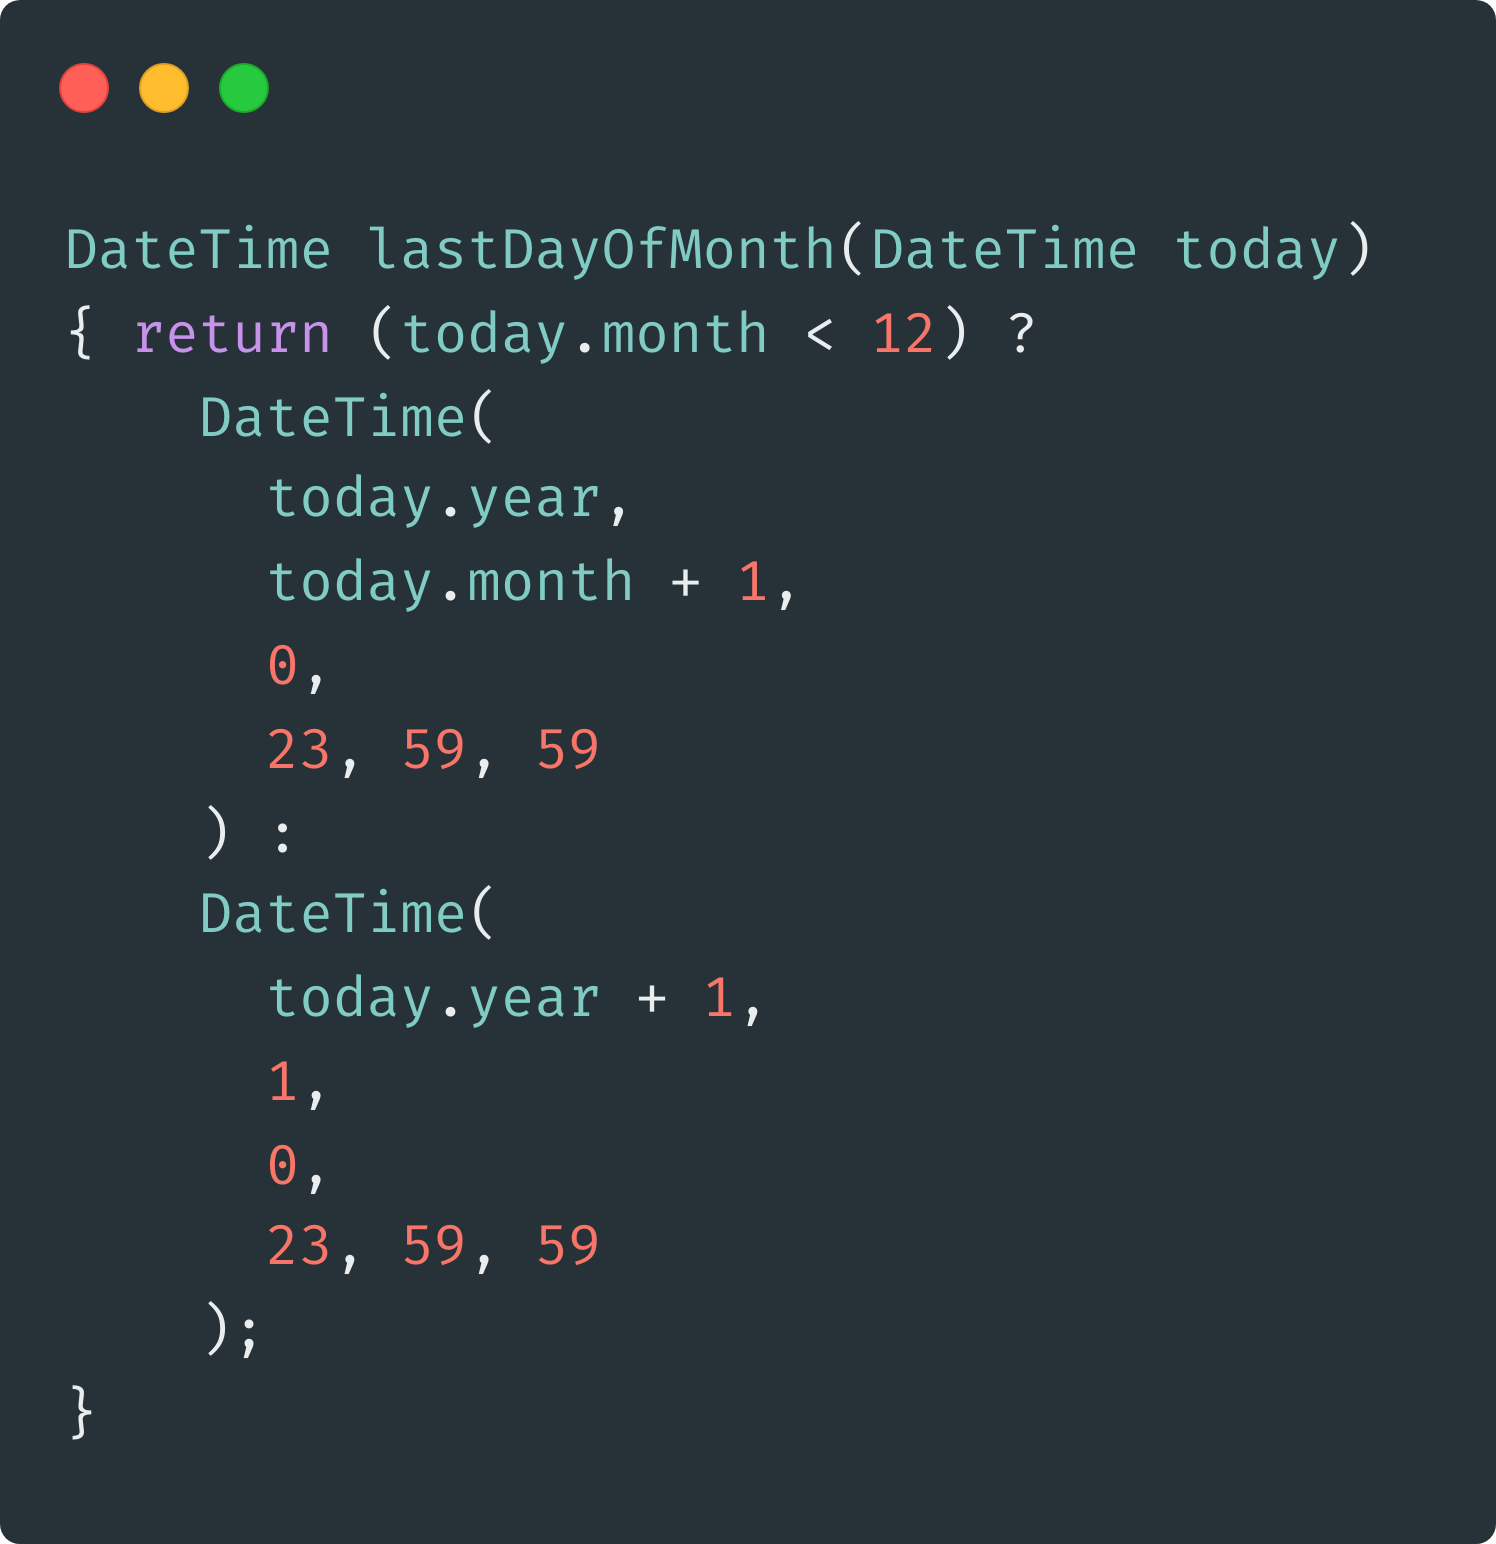
\includegraphics[width=0.6\columnwidth]{last_day_of_month}
    \caption{Dart: Letzter Tag des Monats}
\end{figure}

